\documentclass[020-persona\_validation.tex]{subfiles}

\begin{document}

    % TODO calculate and fill in these numbers
    There were a total of 68 responses to the persona survey.
    %**** were over 18 years old and also consented to the research study.
    57 complete observations % from 010-prep_survey_questions.R: dim(wide_survey_likert)
    were used for the factor analysis, Cronbach's alpha, and clustering analysis.
    %of the ***** incomplete responses,
    %**** completed ****\% of the survey.
    The persona survey had 1 set of responses % 01-process_qualtrics.R
    that shared a duplicate ID.
    Looking at the individual responses,
    it was determined that this particular set of IDs came from the same person.
    Duplicate responses were back filled for any missing values (i.e., coalesced),
    and only the initial set of responses were kept for analysis.
    % from 03-pca_clustering saved to data/final/paper/num_obs_clustering.RDS
    57 complete observations % 03-pca_clustering.Rmd; uses data from validation
    were used for clustering.

    Items from exploratory factor analysis (EFA) grouped respondents
    using hierarchical clustering with Euclidean distance and Ward's clustering method
    to identify learner personas.
    Overall,
    we used the 3-factor model and the clustering results yielded 3 clusters for our personas.

    \subsection{Survey Study Participants}

        67 survey respondents self-reported their current occupation and career stage.
        These responses were further grouped into 3 overall occupations:
        (1) student,
        (2) researcher, and
        (3) clinician.
        Clinical students were placed in the student category,
        and the ``researcher'' role was a catch-all for all the other responses.
        Figure \ref{fig:groupeddemographics} shows the grouped occupation counts.
        The original ungrouped demographic counts are shown in Supplemental Figure \ref{fig:demographics_occupation}.

        \begin{figure}[!hbtp]
            \centering
            \includegraphics[width=0.5\textwidth]{figs/020-persona/grouped\_demographics.png}
            \caption[Grouped demographics for persona survey respondents]{
            Total number of survey respondents from the persona study and their self-reported occupation.
                This particular survey question was a ``select all that applies''
                question with the ability to type in an ``other'' response.
                The responses were then grouped together into the 3 major occupation groups as shown.}
            \label{fig:groupeddemographics}
        \end{figure}

        Of the 67 respondents,
        29 reported as being a student,
        21 reported as being a clinician, and
        26 were classified as being a researcher.

        Overall (Figure \ref{fig:likert}),
        we count that the respondents agree and strongly agree with the statement
        that having access to raw data is important to be able to repeat an analysis.
        However, they also strongly disagree with the notion that
        they can write small programs to work with data or address a problem with their own work. % TODO does this interpret as and/or?
        They either have neutral or strong agreements towards programming languages (e.g., R, Python, etc)
        making analysis more efficient and easier to reproduce.
        Most respondents were also leaning towards an agreement about being able to search for technical help online.

        % TODO: i think these are enough of the raw responses,
        % TODO: the individual question responses will make more sense to show with the clusters
        \begin{figure}[!hbtp]
            \centering
            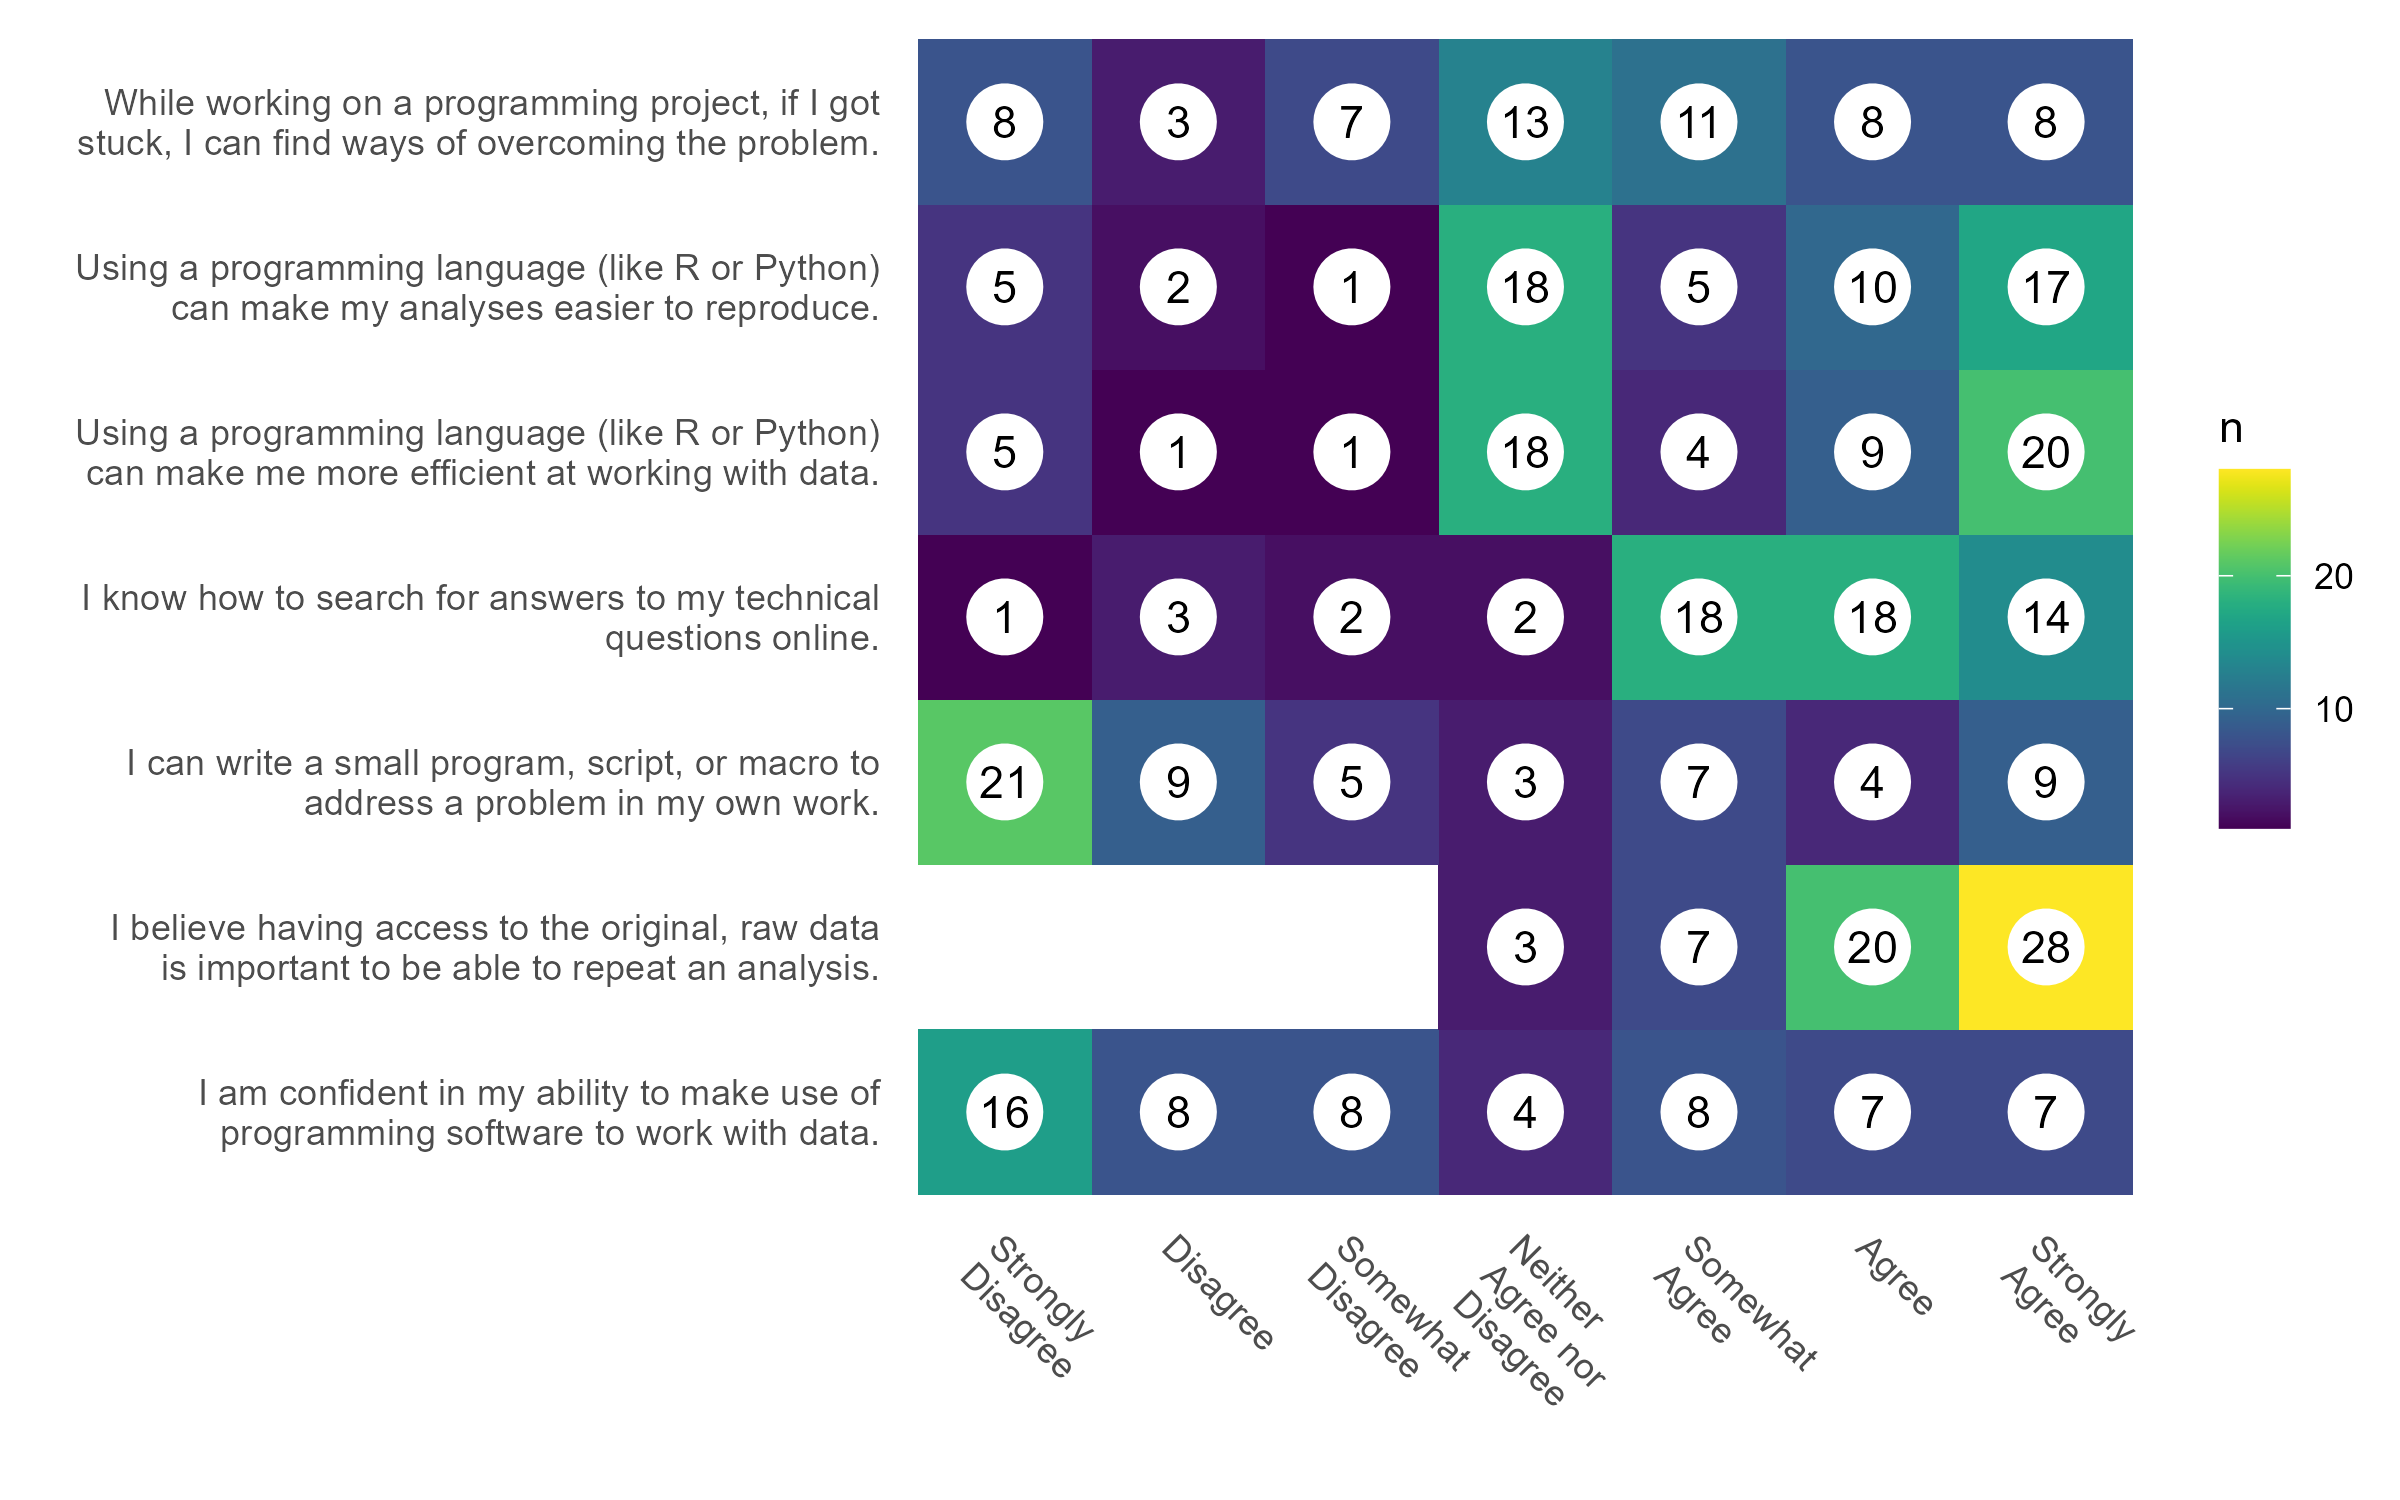
\includegraphics[width=0.95\textwidth]{figs/020-persona/likert.png}
            \caption[Summary Likert scale responses]
            {Number of responses for each summary Likert scale question.
             Likert questions were initially created as a summary table to gauge respondents attitudes programming
             in data analysis.
             Results show that most respondents believe having raw access to data is important to repeat an analysis,
             but are less likely able to use a programming language to perform an analysis.
             There is a bimodal distribution between being indifferent and strongly agreeing
             about programming languages making analysis easier and more efficient.
            }
            \label{fig:likert}
        \end{figure}

    \subsection{Survey Validation}

        Factor Analysis and Cronbah's Alpha was performed on 14 of the the 23 survey items.
        The results were used to validate the survey.
        The clustering for persona identification was performed in a separate step.

    \subsubsection{Factor Analysis}

        Survey items were selected for factor analysis based on its correlation with other variables and their significance
        ($\left|\rho\right| \ge 0.5$ and $p < 0.05$).
        Figure \ref{fig:persona-item-corr} shows the correlation matrix between all items.
        (only significant correlations are shown).
        Items with a high correlation coefficient ($\left|\rho\right| \ge 0.5$) were candidates to be selected for factor analysis.
        Item candidates that were both significant and highly correlated with at least 20\% of the other items were
        selected for factor analysis.
        These parameters reduced the number of items for factor analysis,
        while still keeping at least 1 item from each section of the survey.

        \begin{figure}[!hbtp]
            \centering
            \includegraphics[width=0.9\textwidth]{figs/010-validation/efa\_item\_correlations.png}
            \caption[Correlation matrix of persona items]
            {Correlation plot of all the items in the persona survey.
             Plot uses the same variable ordering as the clustering analysis,
             hierarchical clustering with Euclidean distance using Ward's (ward.D2) clustering method.
             Only significant correlations are shown ($p < 0.05$).
             Items that had a high correlation coefficient ($\left|\rho\right| \ge 0.5$)
             were candidates to be used for factor analysis.
            }
            \label{fig:persona-item-corr}
        \end{figure}

        14 items met the criteria for factor analysis.
        The scree plot (Figure \ref{fig:scree-fa-good}) suggested testing factor models between two (2) and four (4) factors
        (Supplemental Figure \ref{fig:scree-fa-all} shows the scree plot for all the survey items).

        \begin{figure}[!hbtp]
            \centering
            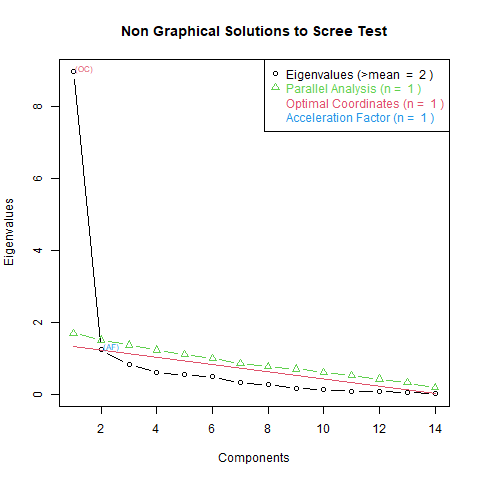
\includegraphics[width=0.5\textwidth]{figs/010-validation/efa_eigen_scree_good.png}
            \caption[Scree plot for factor analysis]
            {Scree plot for factor analysis showing the number of components (x) and the eigenvalues (y).
                The figure suggests exploring 2 to 4-factor models.
            }
            \label{fig:scree-fa-good}
        \end{figure}

        % TODO: This is done to check for the normality of the data. If the data are normally distributed, we may use maximum
        % likelihood (ML) for the EFA, which will allow more detailed analysis. Otherwise, the extraction method of
        % choice is principal axis factoring (PAF), because it does not require normally distributed data (Brown, 2015).
        % TODO: cite: https://wnarifin.github.io/workshop/qvw2017/efa.pdf
        A 3-factor model was chosen based on
        varimax rotation and
        ``ten Berge'' scores.
        The type of rotation did not affect the results.
        The biggest differences occurred with the number of factors and factoring method.

        The maximum likelihood (ML) factoring method was ruled out because data was not normally distributed
        as confirmed by Q-Q plots and Shapiro Wilk's tests for teach item. % (Supplemntal \ref{ss:fa-data-normality}).
        The 3-factor model had the most interpretability, and was used for the final model.
        Multiple factoring methods were tested using the 3-factor model,
        outside of the ML factoring method, the minimum chi-square (minchi) method had the lowest BIC score,
        and also had good cutoff values (TIL > 0.9, RMSEA < 0.08).
        However, a slightly lower fit model (TIL = 0.93, RMSEA = 0.09) using principal axis factoring (PA)
        was chosen because it better suited our data
        (Table \ref{tab:all-good-3fa-varimax-models}, \ref{tab:all-good-varimax-models})
        \cite{arifinExploratoryFactorAnalysis2017, brownConfirmatoryFactorAnalysis2015}.

        % latex table generated in R 4.1.1 by xtable 1.8-4 package
        % Tue Oct 26 22:33:54 2021
        \begin{table}[!hbtp]
            \centering
            \caption[Factoring methods for 3-factor model cutoffs]
            {Cuttoff scores sorted by BIC for all 3-factor varimax rotated models.
             The maximum likelihood (ML) and minimum chi-square (minchi) factoring methods
             had the best cutoff values,
             but both had to be ruled out because the methods were not suitable for the data.
             Principal axis factoring (PA) was choosen because it does not require normally distributed data
             \cite{arifinExploratoryFactorAnalysis2017, brownConfirmatoryFactorAnalysis2015}.
             Only varimax rotations are shown, since the rotation did not change any of the cutoff scores,
             even when comparing orthogonal rotations to oblique transformations.
            }
            \begin{tabular}{rcllrrr}
                \hline
                & nfactors & rotation & fm & tli & rmsea & bic \\
                \hline
                1 &   3 & varimax & ml & 0.98 & 0.05 & -151.18 \\
                2 &   3 & varimax & minchi & 0.97 & 0.06 & -145.35 \\
                3 &   3 & varimax & old.min & 0.94 & 0.09 & -134.97 \\
                4 &   3 & varimax & uls & 0.93 & 0.09 & -130.59 \\
                5 &   3 & varimax & ols & 0.93 & 0.09 & -130.59 \\
                6 &   3 & varimax & minres & 0.93 & 0.09 & -130.59 \\
                7 &   3 & varimax & pa & 0.93 & 0.09 & -130.58 \\
                8 &   3 & varimax & minrank & 0.92 & 0.10 & -126.12 \\
                9 &   3 & varimax & alpha & 0.91 & 0.11 & -124.42 \\
                10 &   3 & varimax & wls & 0.84 & 0.14 & -96.67 \\
                11 &   3 & varimax & gls & 0.81 & 0.16 & -82.37 \\
                \hline
            \end{tabular}
            \label{tab:all-good-3fa-varimax-models} % good means good variable combinations
        \end{table}

        % latex table generated in R 4.1.1 by xtable 1.8-4 package
        % Tue Oct 26 16:43:21 2021
        \begin{table}[!hbtp]
            \centering
            \caption[Factoring methods for all factor methods]
            {
                All varimax rotation factor analysis models that met cutoff values of
                $\text{TLI} \ge 0.9$ and $\text{RMSEA} < 0.08$ sorted by BIC.
                The 4-factor model had less interpretability than the 3-factor model.
                However, the maximum likelihood and minimum chi-squarefactoring methods of the
                3-factor model did not suit the data
                \cite{arifinExploratoryFactorAnalysis2017, brownConfirmatoryFactorAnalysis2015}.
            }
            \begin{tabular}{rcllrrr}
                \hline
               & nfactors & rotation & fm & tli & rmsea & bic \\
                \hline
                1 &   3 & varimax & ml & 0.98 & 0.05 & -151.18 \\
                2 &   3 & varimax & minchi & 0.97 & 0.06 & -145.35 \\
                3 &   4 & varimax & ml & 1.02 & 0.00 & -130.86 \\
                4 &   4 & varimax & minchi & 1.02 & 0.00 & -130.85 \\
                5 &   4 & varimax & pa & 1.01 & 0.00 & -128.45 \\
                6 &   4 & varimax & minres & 1.01 & 0.00 & -128.33 \\
                7 &   4 & varimax & uls & 1.01 & 0.00 & -128.33 \\
                8 &   4 & varimax & ols & 1.01 & 0.00 & -128.26 \\
                9 &   4 & varimax & alpha & 1.00 & 0.00 & -125.00 \\
                10 &   4 & varimax & old.min & 0.99 & 0.03 & -122.20 \\
                11 &   4 & varimax & minrank & 0.99 & 0.04 & -120.50 \\
                 \hline
              \end{tabular}
            \label{tab:all-good-varimax-models} % good means good variable combinations
        \end{table}

        The results in Table \ref{tab:fa-3} show the item loadings for the 3-factor model.
        The factors can be interpreted as
        programming experience (PA1),
        statistics confidence (PA2), and
        programming for data analysis (PA3).

        % Table generaged from the 05-fa_cart.Rmd file
        % latex table generated in R 4.1.1 by xtable 1.8-4 package
        % Mon Oct 18 13:21:58 2021
        \begin{table}[!hbtp]
            \centering
            \caption[3-factor item loadings]
            {Factor loadings, communality, uniqueness, and complexity
                based on minimum sample size weighted chi square factoring method with varimax rotation and tenBerge scores.
                The three factors are:
                programming experience (PA1),
                programming for data analysis (PA2), and
                solving technical problems (PA3).
                Loadings $<$ 0.5 are suppressed.
                Loadings $\ge$ to 0.6 were used for Cronbah's $\alpha$.
            }
            \begin{tabular}{rllllrrr}
                \hline
               & item & PA1 & PA2 & PA3 & Communality & Uniqueness & Complexity \\
                \hline
              1 & Q3.4 & 0.811 &  &  & 10.34 & 0.17 & 1.54 \\
                2 & Q3.3 & 0.799 &  &  & 10.34 & 0.13 & 1.75 \\
                3 & Q7.2\_2 & 0.793 &  &  & 10.34 & 0.13 & 1.78 \\
                4 & Q3.5 & 0.774 &  &  & 10.34 & 0.16 & 1.82 \\
                5 & Q3.1 & 0.729 &  &  & 10.34 & 0.17 & 2.12 \\
                6 & Q7.2\_5 & 0.695 &  &  & 10.34 & 0.25 & 2.08 \\
                7 & Q5.2 & 0.682 &  &  & 10.34 & 0.35 & 1.73 \\
                8 & Q4.3 &  &  &  & 10.34 & 0.56 & 2.36 \\
                9 & Q7.2\_7 &  & 0.944 &  & 10.34 & 0.02 & 1.19 \\
                10 & Q7.2\_6 &  & 0.87 &  & 10.34 & 0.07 & 1.45 \\
                11 & Q4.2 &  &  & 0.718 & 10.34 & 0.40 & 1.32 \\
                12 & Q7.2\_3 &  &  & 0.64 & 10.34 & 0.31 & 2.26 \\
                13 & Q6.1 &  &  & 0.538 & 10.34 & 0.60 & 1.68 \\
                14 & Q7.2\_4 & 0.506 &  & 0.509 & 10.34 & 0.33 & 2.85 \\
                 \hline
              \end{tabular}
            \label{tab:fa-3}
        \end{table}

    \subsubsection{Cronbah's Alpha}

        Internal consistency was measured with Cronbah's alpha.
        A separate Alpha was calculated from each of the factor analysis results.
        Questions that had a loading above $0.6$ was used for the alpha calculation.
        The $0.6$ cutoff was mainly selected to make sure all the major question groups in the survey was represented
        and each factor had more than 1 question.
        The programming experience subscale (PA1) consisted of 7 items ($\alpha = 0.96$),
        the programming for data analysis (PA2) consisted of 2 items ($\alpha = 0.98$), and
        the solving technical problems subscale (PA3) consisted of 2 items ($\alpha = 0.75$).

    \subsection{Clustering and Persona Identification}

        Hierarchical clustering was used on all 23 survey items to identify personas.
        Clusters were combined with survey demographic and item responses to create the learner personas.
        Questions with high factor loadings along with demographic results were used to guide the clustering interpretations
        (Figure \ref{fig:cluster-results}).

    \subsubsection{Clustering}

        The agglomerative coefficient was used to select Ward's clustering method (0.88) over
        average (0.54), single (0.37), and complete (0.72).
        The total within-cluster sum of squares was used to generate an elbow plot (Figure \ref{sfig:cluster-elbow})
        and gap statistic for different numbers of clusters (Figure \ref{sfig:cluster-gap}).
        These results were were used to
        determine that three (3) clusters were the most optimal number of clusters.
        Three (3) clusters were and also the most interpretable
        (Figure \ref{fig:cluster-gap-elbow}).
        The dendrogram of the three (3) clusters are shown in
        Supplemental Figure \ref{fig:dendro-cluster-3}.

        %gap statistic: https://web.stanford.edu/~hastie/Papers/gap.pdf
        % TODO: the subfigures are not showing up in the figure listing
        \begin{figure}[!hbtp]
            \centering
            \begin{subfigure}[h]{0.45\textwidth}
                \centering
                \includegraphics[scale=0.4]{figs/020-persona/elbow\_plot-survey\_likert.png}
                \caption[Elbow plot for determining optimal number of clusters.]
                {Elbow plot showing the total within-cluster sum of squares (y-axis) for increasing number of clusters, k (x-axis).
                }
                \label{sfig:cluster-elbow}
            \end{subfigure}
            \begin{subfigure}[h]{0.45\textwidth}
                \centering
                \includegraphics[scale=0.4]{figs/020-persona/gap\_statistic-survey\_likert.png}
                \caption[Gap statistic for determining optimal number of clusters.]
                {Gap statistic comparing
                    intra-cluster variation as compared to a distribution with no clustering (y-axis)
                    for different number of clusters, k (x-axis).
                }
                \label{sfig:cluster-gap}
            \end{subfigure}
            \caption[Elbow plot and Gap statistic for optimal number of clusters.]
            {Determining the number of optimal clusters for the persona survey data.
                Each cluster would become a learner persona.
                (\ref{sfig:cluster-elbow}) shows the elbow plot for the data and
                suggests that the optimal number of clusters is between $k=2$ and $k=4$.
                (\ref{sfig:cluster-gap}) shows the gap statistic for the data.
                The dotted line at $k=3$ shows the optimal number of k clusters.
                The three (3) cluster model had the best interpretation from the survey data.
                Each cluster became its own learner persona.
            }
        \label{fig:cluster-gap-elbow}
        \end{figure}

    \subsubsection{Persona Identification}

        % TODO: 67 values in persona, 57 had a cluster group value
        Results from clustering were incorporated into the survey results in order to identify learner personas
        (Figure \ref{fig:cluster-results}).
        The highest loaded item in each factor
        (Figures \ref{sfig:cluster-q3-4}, \ref{sfig:cluster-q7-2-7}, \ref{sfig:cluster-q4-2})
        and the occupations demographic breakdowns
        (Figure \ref{sfig:cluster-grouped-demogrphics})
        give an overview of the clusters.

        Clinicians (the target audience) were primarily in Groups 1 and 3.
        There were no students in Group 3.
        Groups 1 and 2 were spread out across the 3 occupations,
        however,
        Group 2 had the fewest number of clinicians (Figure \ref{sfig:cluster-grouped-demogrphics}).
        Group 3 were either clinicians or academics, with most of the Group 3 occupations being a clinician.
        Original ungrouped occupation breakdown are shown in Supplemental Figure \ref{fig:demographics_occupation_cluster}.

        Looking at programming experience
        (Q3.4, Figure \ref{sfig:cluster-q3-4}),
        Group 2 had the most amount of experience
        and Groups 1 and 3 were predominately ``never'' programmers.
        Group 2 had the most number of respondents strongly agreeing to the statement that
        using a programming language can make an analysis easier to reproduce
        (Q 7.2-7, Figure \ref{sfig:cluster-q7-2-7}).
        Groups 1 and 3 are mostly neutral towards the statement and are the only respondents who disagree and strongly disagree
        with the statement.
        Looking at solving technical questions
        (Q4.2, Figure \ref{sfig:cluster-q4-2}).

        \begin{figure}[!hbtp]
            \centering
            \begin{subfigure}[h]{0.45\textwidth}
                \centering
                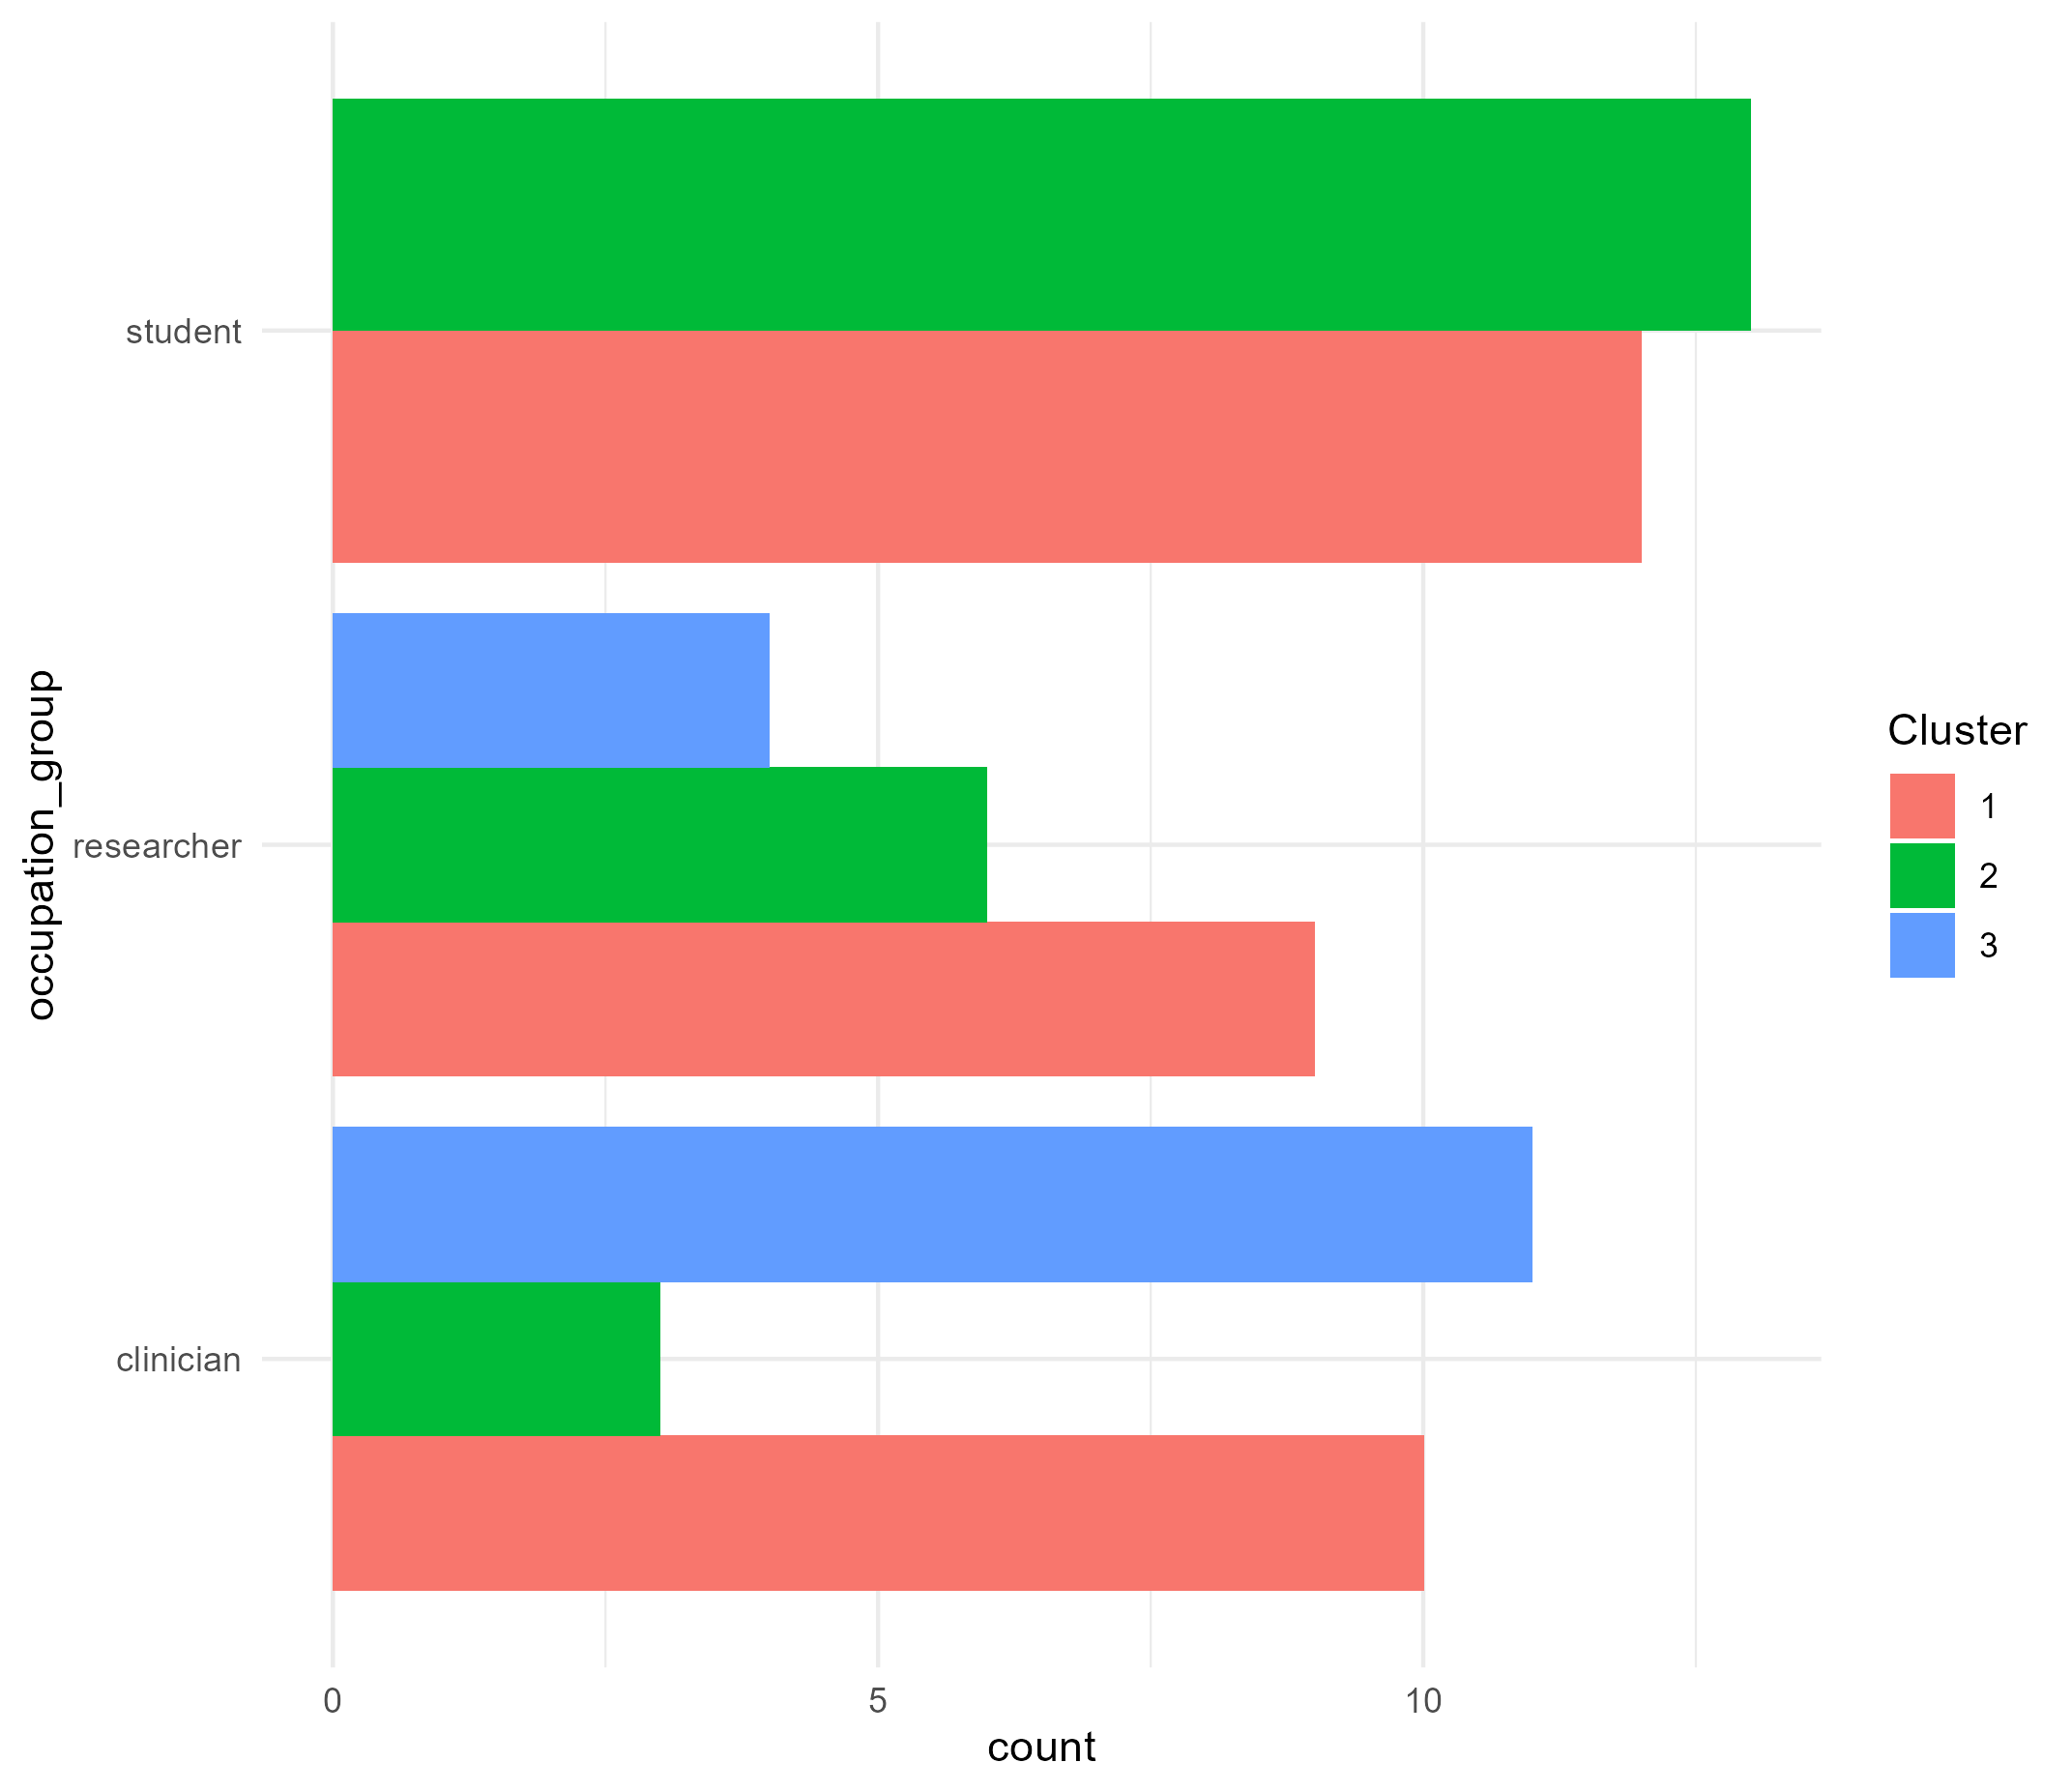
\includegraphics[scale=0.35]{figs/020-persona/survey\_likert/group_cluster_occupation_3.png}
                \caption[Grouped demographics for 3 clusters]
                {Grouped demographics for 3 clusters.
                }
                \label{sfig:cluster-grouped-demogrphics}
            \end{subfigure}
            \begin{subfigure}[h]{0.45\textwidth}
                \centering
                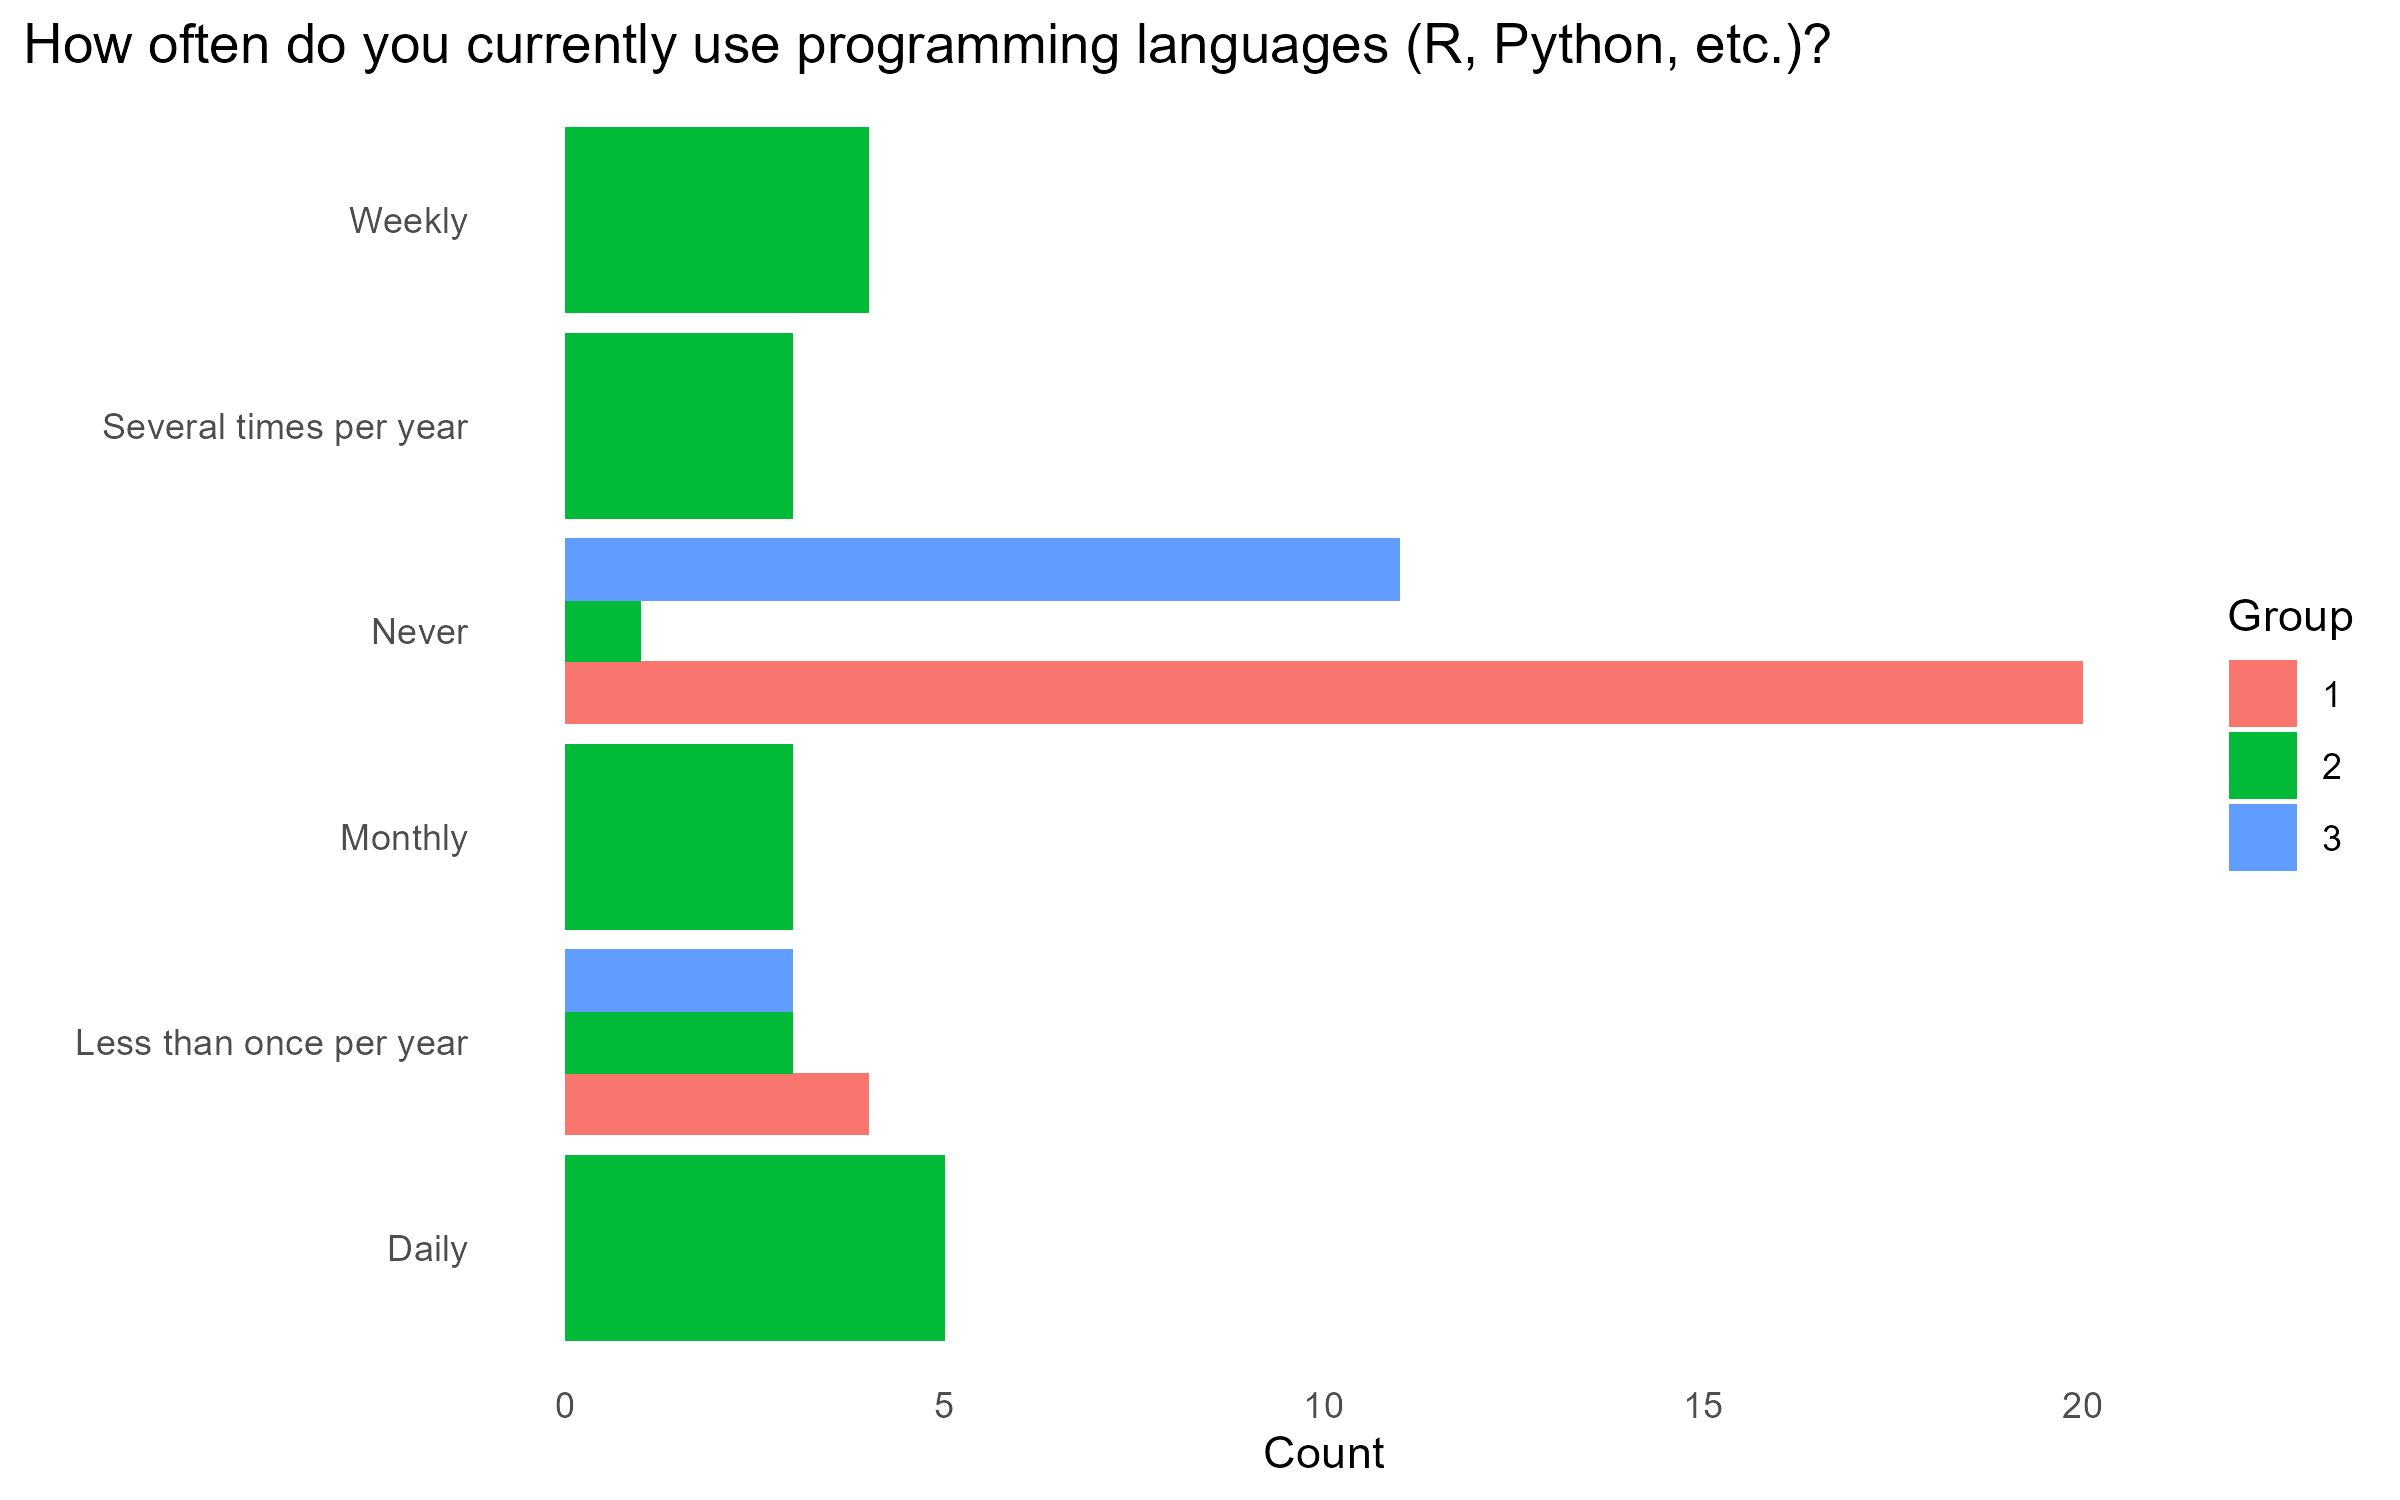
\includegraphics[scale=0.35]{figs/020-persona/survey\_likert/Q3.4-group-3.png}
                \caption[How often do you program (Q3.4) for 3 clusters]
                {Clustered responses for Q3.4: Programming experience factor.
                ``How often do you currently use programming languages (R Python, etc.)?''.}
                \label{sfig:cluster-q3-4}
            \end{subfigure}
            \begin{subfigure}[h]{0.45\textwidth}
                \centering
                \includegraphics[scale=0.35]{figs/020-persona/survey\_likert/Q7.2\_7-3.png}
                \caption[Data programming Q7.2-7 for 3 clusters.]
                {Clustered responses for Q7.2-7: Programming for analysis factor.
                ``Using a programming language (like R or Python) can make my analyses easier to reproduce.''}
                \label{sfig:cluster-q7-2-7}
            \end{subfigure}
            \begin{subfigure}[h]{0.45\textwidth}
                \centering
                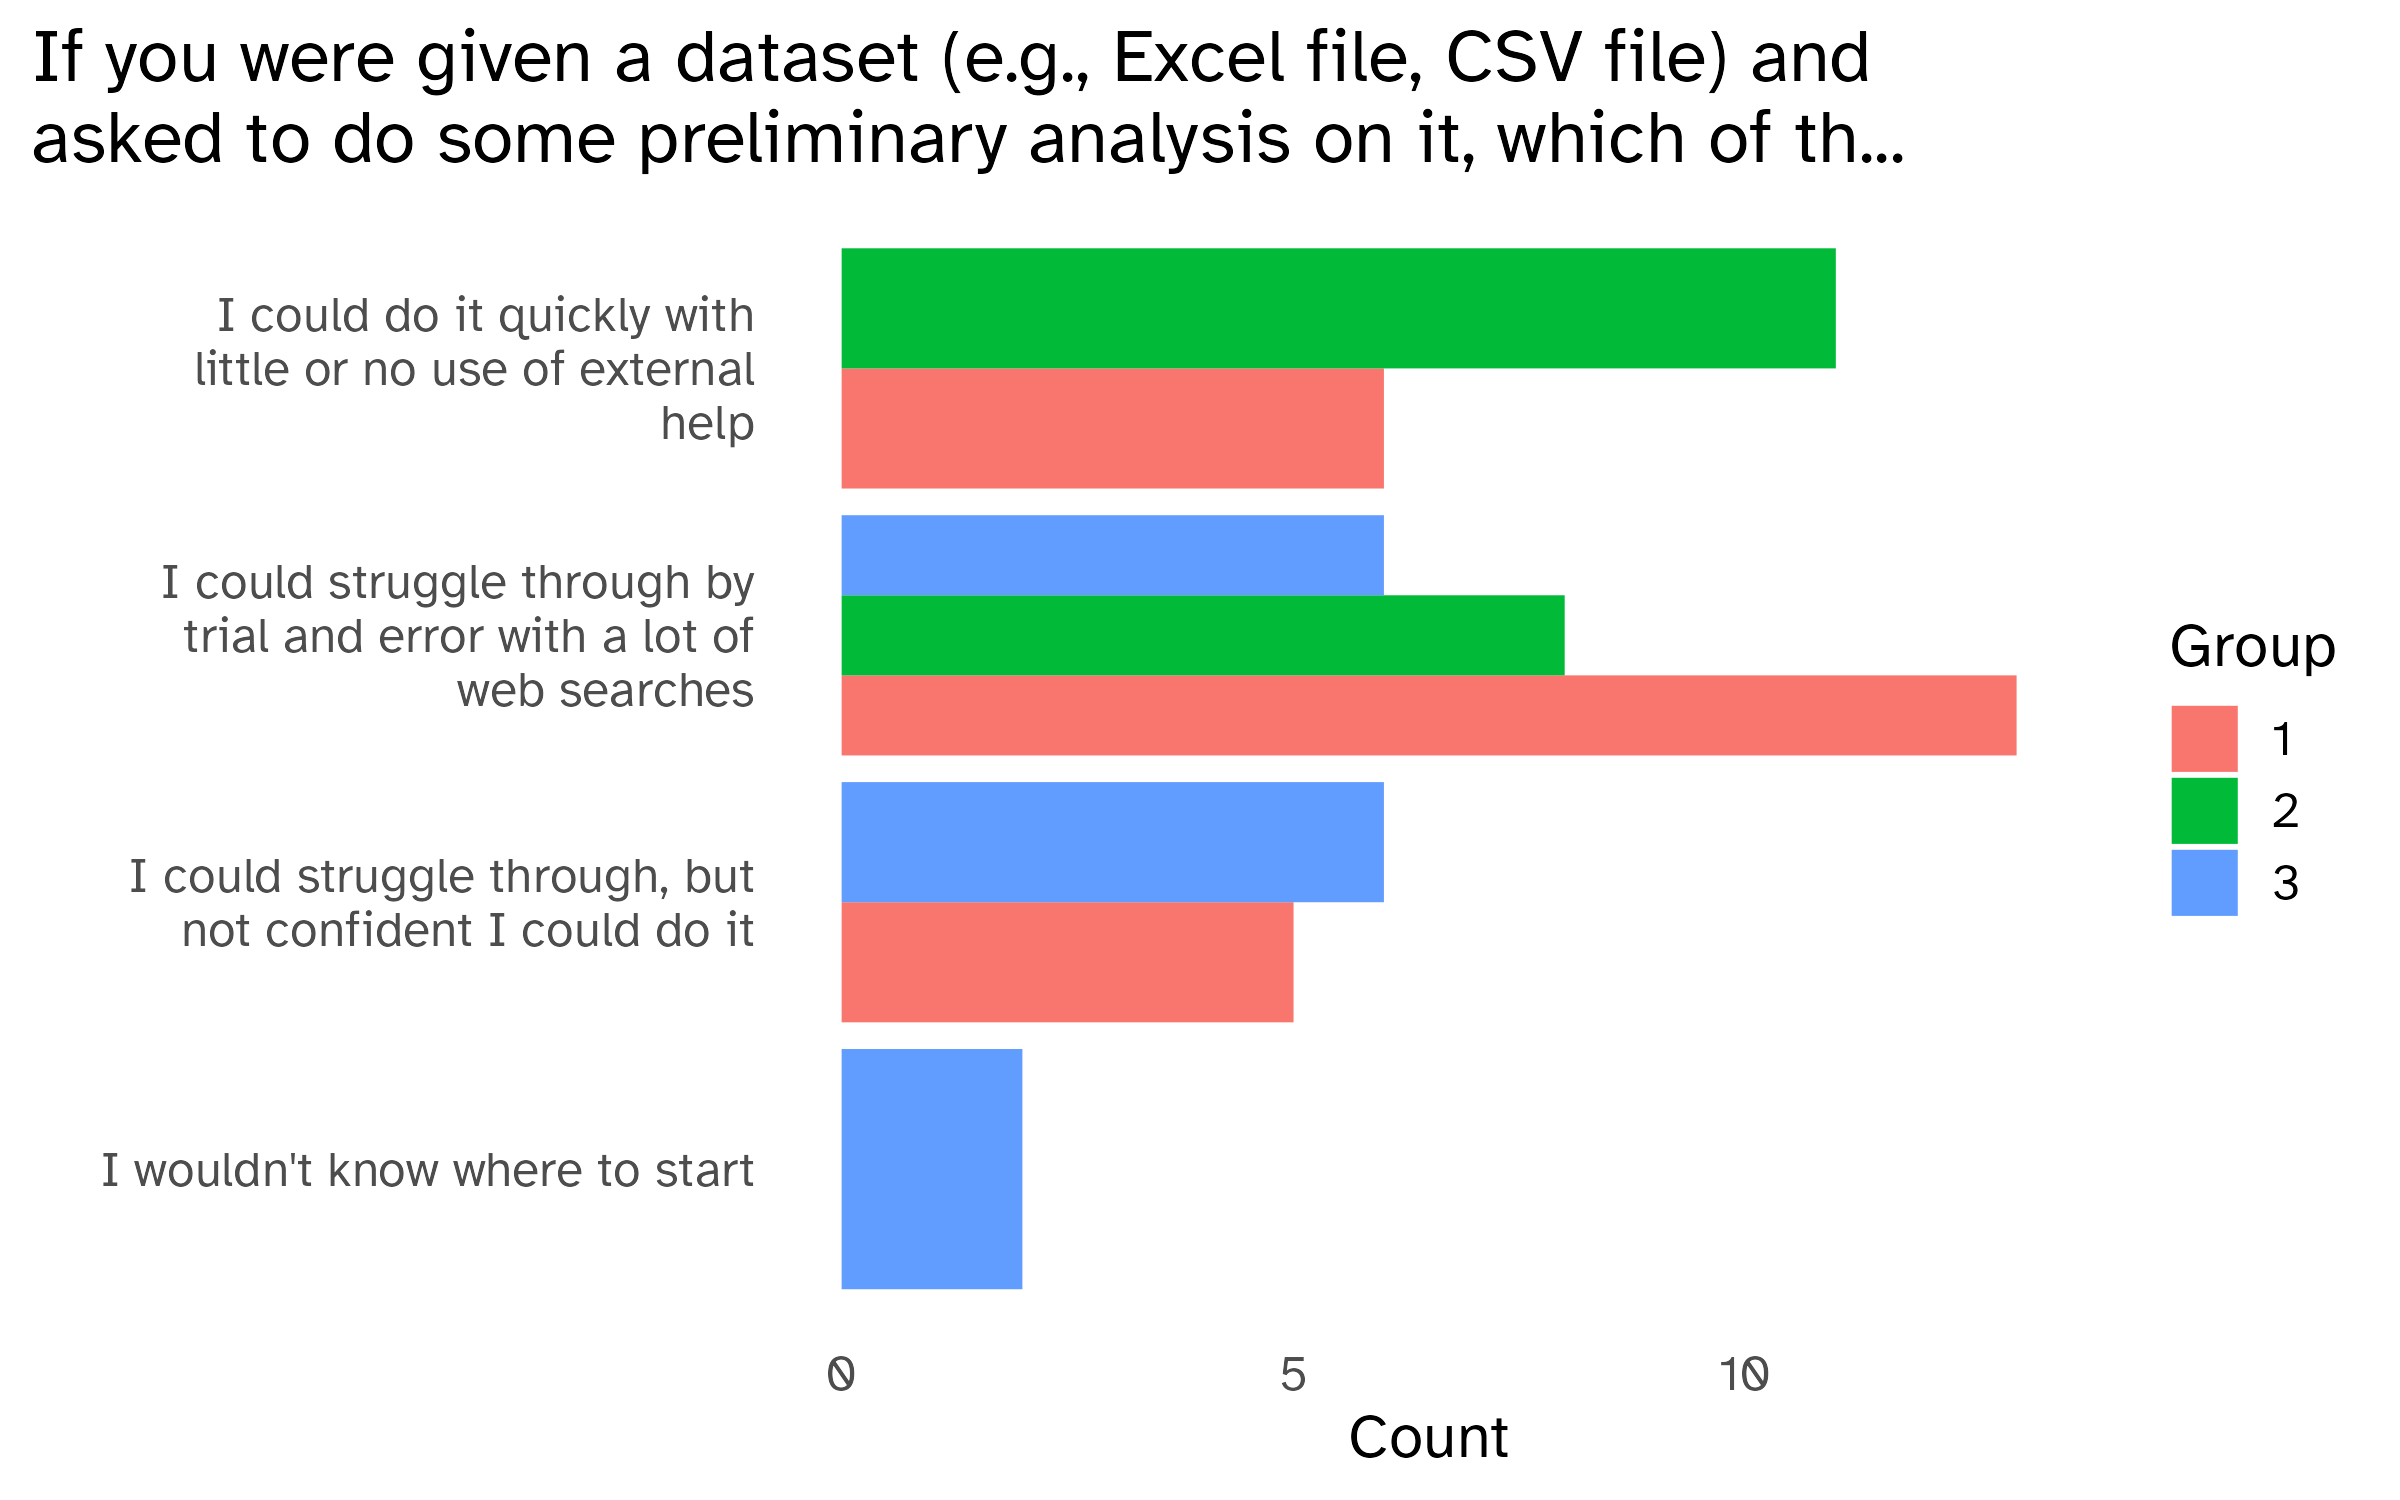
\includegraphics[scale=0.35]{figs/020-persona/survey\_likert/Q4.2-group-3.png}
                \caption[Statistics question for logistic regression (Q6.2) for 3 clusters]
                {Clustered responses for Q4.2: Solving technical problems factor.
                ``If you were given a dataset (e.g., Excel file, CSV file) and asked to do some preliminary analysis on it,
                which of these best describe how easily you can accomplish the task?''}
                \label{sfig:cluster-q4-2}
            \end{subfigure}
            \caption[Selected survey questions for 3 clusters]
            {Survey responses for each of the 3 clusters.
                (\ref{sfig:cluster-grouped-demogrphics})
                Group 1 and 3 had common demographics, However Group 1 also included students.
                Group 3 had the most number of clinicians.
                Group 2 were predominantly students.
                (\ref{sfig:cluster-q3-4})
                Group 2 are more consistent users of programming languages than Group 1 and 3.
                (\ref{sfig:cluster-q7-2-7})
                Results show the likert table responses for each of the 3 groups.
                Group 2 feel programming will make analyses easier to reproduce than Group 1 and 3.
                (\ref{sfig:cluster-q4-2})
                Group 3 were the only group of people who did not how to start an analysis.
                Group 2 had the most number of responses for being able to do the analysis with minimal help.
                These results were similar to the question that asked a more specific statistics related question
                (Supplemental Figure \ref{sfig:cluster-q6-2})
            }
            \label{fig:cluster-results}
        \end{figure}

        The 2-cluster results did not provide enough details between our participants.
        The major splits were the student group (Group 2 in the 3 cluster results) and everyone else.
        In the 4-cluster results
        (Supplemental Figure \ref{fig:dendro-4}),
        the additional split occurred in the student group.
        This split was difficult to interpret and the new cluster was unable to be distinguished from the other split group.

    \subsubsection{Persona Creation}

        Using the clustering data (Supplemental Figure \ref{fig:dendro-cluster-3})
        with the survey results, three (3) learner personas were created:
        Ash Academic (Group 1), Samir Student (Group 2), Claire Clinician (Group 3).
        Each persona had 4 components: (1) background, (2) relevant prior knowledge or experience,
        (3) perception of needs, and (4) special considerations
        \cite{rstudioLearnerPersonas2019, softwarecarpentryLearnerProfiles, wilson2019teaching}.
        The results from the survey were used to write out the
        relevant prior knowledge or experience and perception of needs sections.
        The background and special considerations were written to make each learner persona more complete
        \cite{pruittPersonaLifecycleKeeping2006}.
        Full write-ups with each persona's
        background, relevant prior knowledge or experience, perception of needs, and special considerations
        can be found in Supplemental \ref{sse:learner-personas}.

\end{document}
